\documentclass[tikz,border=3mm]{standalone}

% line thickness
\tikzset{every picture/.style={line width=1pt}}

\tikzset{
  dot/.style={circle, fill=black, minimum size=#1,
                inner sep=0pt, outer sep=0pt},
  dot/.default={5pt}, % default size of the circle diameter 
}

% number of vertices
\def\n{10}

% radius of circle
\def\r{2}

\begin{document}

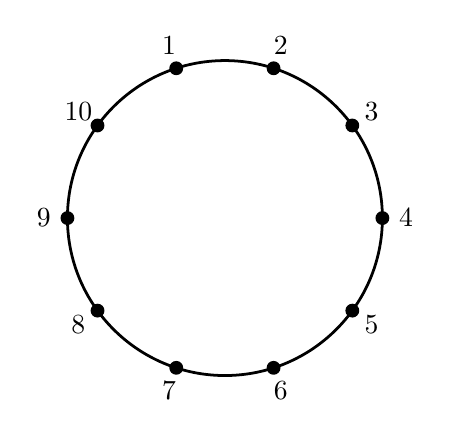
\begin{tikzpicture}
  % draw equidistant points and arc | shifted 3 sectors anti-clockwise with +3*360/\n
  \foreach \x [count=\p] in {0,...,\the\numexpr\n-1\relax} {
      \node[dot] (\p) at (+3*360/\n-\x*360/\n:\r) {};
      \draw (+3*360/\n-\x*360/\n:\r+.3) node {\p};
  };
  % draw circle | using node (4) after the shift
  \draw (4) arc (0:360:\r);
\end{tikzpicture}

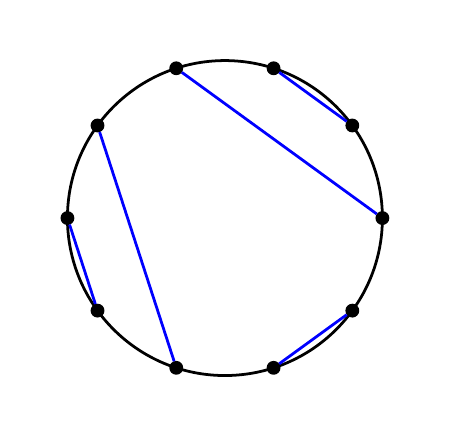
\begin{tikzpicture}
  % draw equidistant points and arc | not shifted
  \foreach \x [count=\p] in {0,...,\the\numexpr\n-1\relax} {
      \node[dot] (\p) at (-\x*360/\n:\r) {};
      \draw (+3*360/\n-\x*360/\n:\r+.3) node {\phantom{\p}};% hack for consistent size
  };
  % draw circle
  \draw (1) arc (0:360:\r);
  % connect points
  \draw[blue] (9) -- (10);
  \draw[blue] (8) -- (1);
  \draw[blue] (7) -- (4);
  \draw[blue] (6) -- (5);
  \draw[blue] (2) -- (3);
\end{tikzpicture}

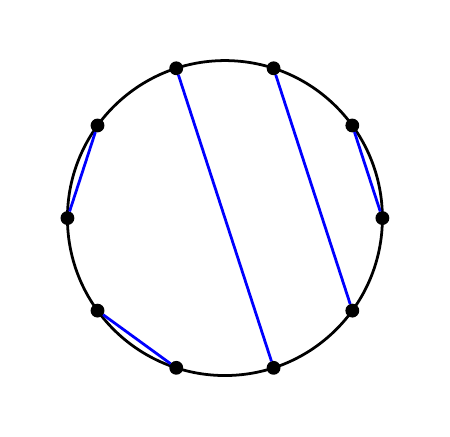
\begin{tikzpicture}
  % draw equidistant points and arc | not shifted
  \foreach \x [count=\p] in {0,...,\the\numexpr\n-1\relax} {
      \node[dot] (\p) at (-\x*360/\n:\r) {};
      \draw (+3*360/\n-\x*360/\n:\r+.3) node {\phantom{\p}};% hack for consistent size
  };
  % draw circle
  \draw (1) arc (0:360:\r);
  % connect points
  \draw[blue] (5) -- (4);
  \draw[blue] (7) -- (6);
  \draw[blue] (8) -- (3);
  \draw[blue] (9) -- (2);
  \draw[blue] (10) -- (1);
\end{tikzpicture}

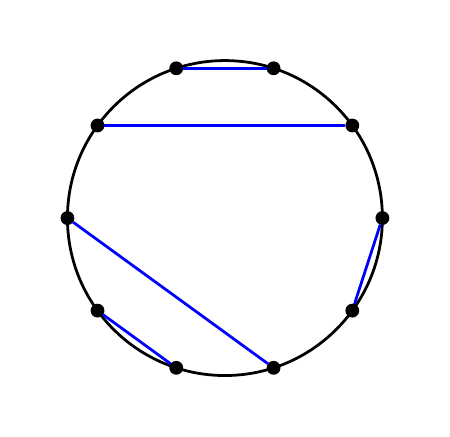
\begin{tikzpicture}
  % draw equidistant points and arc | not shifted
  \foreach \x [count=\p] in {0,...,\the\numexpr\n-1\relax} {
      \node[dot] (\p) at (-\x*360/\n:\r) {};
      \draw (+3*360/\n-\x*360/\n:\r+.3) node {\phantom{\p}};% hack for consistent size
  };
  % draw circle
  \draw (1) arc (0:360:\r);
  % connect points
  \draw[blue] (5) -- (4);
  \draw[blue] (6) -- (3);
  \draw[blue] (1) -- (2);
  \draw[blue] (8) -- (9);
  \draw[blue] (7) -- (10);
\end{tikzpicture}

\end{document}
